\section{Verification of numerical model}
We chose two well-known instabilities for testing our code: the two stream instability and the Weibel instability. Electromagnetic two stream instability is caused by two fluxes of electrons moving in opposite directions. Modes with the wave vector, normal to electron velocities, grow with the increment $\frac {v}{c}\frac{\omega_{p}}{\sqrt{\gamma}}$, where $\omega_{p}$ is the electron plasma frequency and $\gamma$ is the gamma-factor of both electron fluxes. We study the case with electron velocity $v=0.99c$. As shown in Figure \ref{twostream} magnetic energy growth is very similar to linear growth with analytically computed increment. When the fraction of the magnetic energy becomes close to 10 percent of the full initial energy, the instability reaches its saturation limit. The total energy deviation at the end of the simulation does not exceed 5 percent of the instability energy.
\begin{figure}[h!]
	\centering
	\begin{minipage}{0.49\textwidth}
		%\center{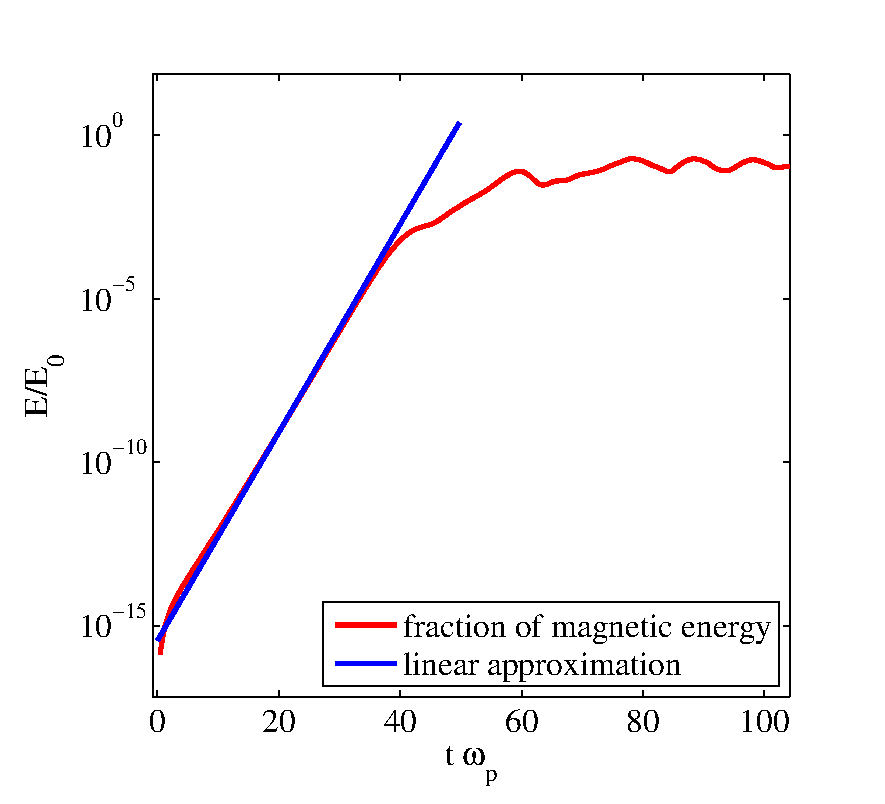
\includegraphics[width=0.99\linewidth]{twostream.eps}}
		\caption{Time dependence of the ratio of the magnetic energy to the full initial energy  in case of the two stream instability.}
		\label{twostream}
	\end{minipage}\hfill
	\begin{minipage}{0.49\textwidth}
		%\center{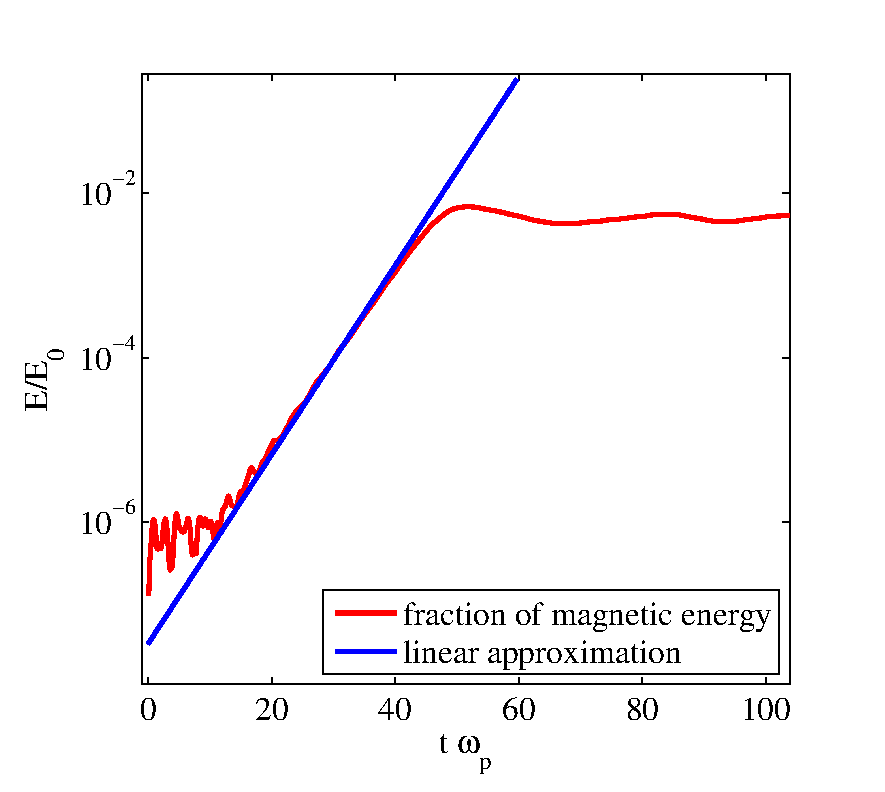
\includegraphics[width=0.99\linewidth]{weibel.eps}}
		\caption{Time dependence of the ratio of the magnetic energy to the full initial energy  in case of the Weibel instability.}
		\label{weibel}
	\end{minipage}
\end{figure}

The second test of the code is the Weibel instability \cite{Weibel1959}, which occurs when the temperature in one spatial direction is smaller then in the other two. This instability has many different cases, we chose the one which was studied by Yoon et al. \cite{Yoon1987}. In this case electrons have delta distribution in transverse momentum and uniform one in parallel. Electron distribution function is:
\begin{equation}
F\left(p_\perp^2, p_\parallel\right)=\frac{1}{2\pi p_{0\perp}}\delta\left(p_\perp - p_{0\perp}\right)\frac{1}{2p_{0\parallel}}H(p_{0\parallel}^2-p_\parallel^2),
\end{equation}
where $\delta$ is the delta-function, $H$ is the Heaviside function, $p_\perp, p_\parallel$ are momentum of particles in perpendicular and parallel directions , respectively, and $p_{0\perp}, p_{0\parallel}$ are constants which determine dispersion of distribution. Dispersion relation for this case can be directly solved, while the expression for the increment is rather cumbersome and will not be presented here for brevity. As shown in Figure \ref{weibel} the numerical simulation with parameters $p_{0\perp} = 20m_e c$ and $p_{0\parallel} = 2 m_e c$ is in good correspondence with the theory.

These results show that our PIC code gives consistent results in the simulation of plasma instabilities and can be applied to more complicated cases.